%%%%%%%%%%%%%%%%%%%%%%%%%%%%%%%%%%%%%%%%%%%%%%%%%%%%%%%%%%%%%%
% --> INTRODUCCIÓN
%%%%%%%%%%%%%%%%%%%%%%%%%%%%%%%%%%%%%%%%%%%%%%%%%%%%%%%%%%%%%%
\section{Introducción}

Las estructuras lineales de datos se caracterizan porque sus elementos están en secuencia, relacionados en forma lineal, uno luego del otro. Cada elemento de la estructura puede estar conformado por uno o varios subelementos o campos que pueden pertenecer a cualquier tipo de dato, pero que normalmente son tipos básicos.

Una estructura lineal de datos o lista está conformada por ninguno, uno o varios elementos que tienen una relación de adyacencia ordenada donde existe un primer elemento, seguido de un segundo elemento y así sucesivamente hasta llegar al último. El tipo de dato de los elementos puede ser cualquiera, pero debe ser el mismo tipo para todos. El valor contenido en los elementos puede ser el mismo o diferente. En estas estructuras se realizan operaciones de agregar y/o eliminar elementos a la lista según un criterio particular. Sobre la base de la forma y el lugar de la realización de estas operaciones en la misma, las listas se clasifican en listas de acceso restringido y listas de acceso no restringido. 

En este laboratorio se trabaja con este tipo de estructuras para implementar listas con arreglos y listas con punteros con nodos simples y dobles.



%%%%%%%%%%%%%%%%%%%%%%%%%%%%%%%%%%%%%%%%%%%%%%%%%%%%%%%%%%%%%%
% --> OBJETIVOS
%%%%%%%%%%%%%%%%%%%%%%%%%%%%%%%%%%%%%%%%%%%%%%%%%%%%%%%%%%%%%%
\subsection{Objetivos}

%%%%%%%%%%%%%%%%%%%%%%%%%%%%%%%%%%%%%%%%%%%%%%%%%%%%%%%%%%%%%%
% --> OBJETIVO GENERAL
%%%%%%%%%%%%%%%%%%%%%%%%%%%%%%%%%%%%%%%%%%%%%%%%%%%%%%%%%%%%%%
\subsubsection{Objetivo General}
\begin{itemize}
\item Hacer uso de plantillas y programación orientada a objetos para la implementación de estructuras lineales.
\end{itemize}

%%%%%%%%%%%%%%%%%%%%%%%%%%%%%%%%%%%%%%%%%%%%%%%%%%%%%%%%%%%%%%
% --> OBJETIVOS ESPECÍFICOS
%%%%%%%%%%%%%%%%%%%%%%%%%%%%%%%%%%%%%%%%%%%%%%%%%%%%%%%%%%%%%%
\subsubsection{Objetivos Específicos}
\begin{itemize}
\item Hacer uso de plantillas y programación orientada a objetos para la implementación de listas con arreglos.
\item Hacer uso de plantillas y programación orientada a objetos para la implementación de listas con punteros.
\item Crear la estructura de una lista simplemente enlazada.
\item Crear la estructura de una lista doblemente enlazada.
\item Implementar algoritmos de búsqueda y ordenamiento de estructuras lineales.
\end{itemize}

%%%%%%%%%%%%%%%%%%%%%%%%%%%%%%%%%%%%%%%%%%%%%%%%%%%%%%%%%%%%%%
% --> ENUNCIADO
%%%%%%%%%%%%%%%%%%%%%%%%%%%%%%%%%%%%%%%%%%%%%%%%%%%%%%%%%%%%%%
\newpage

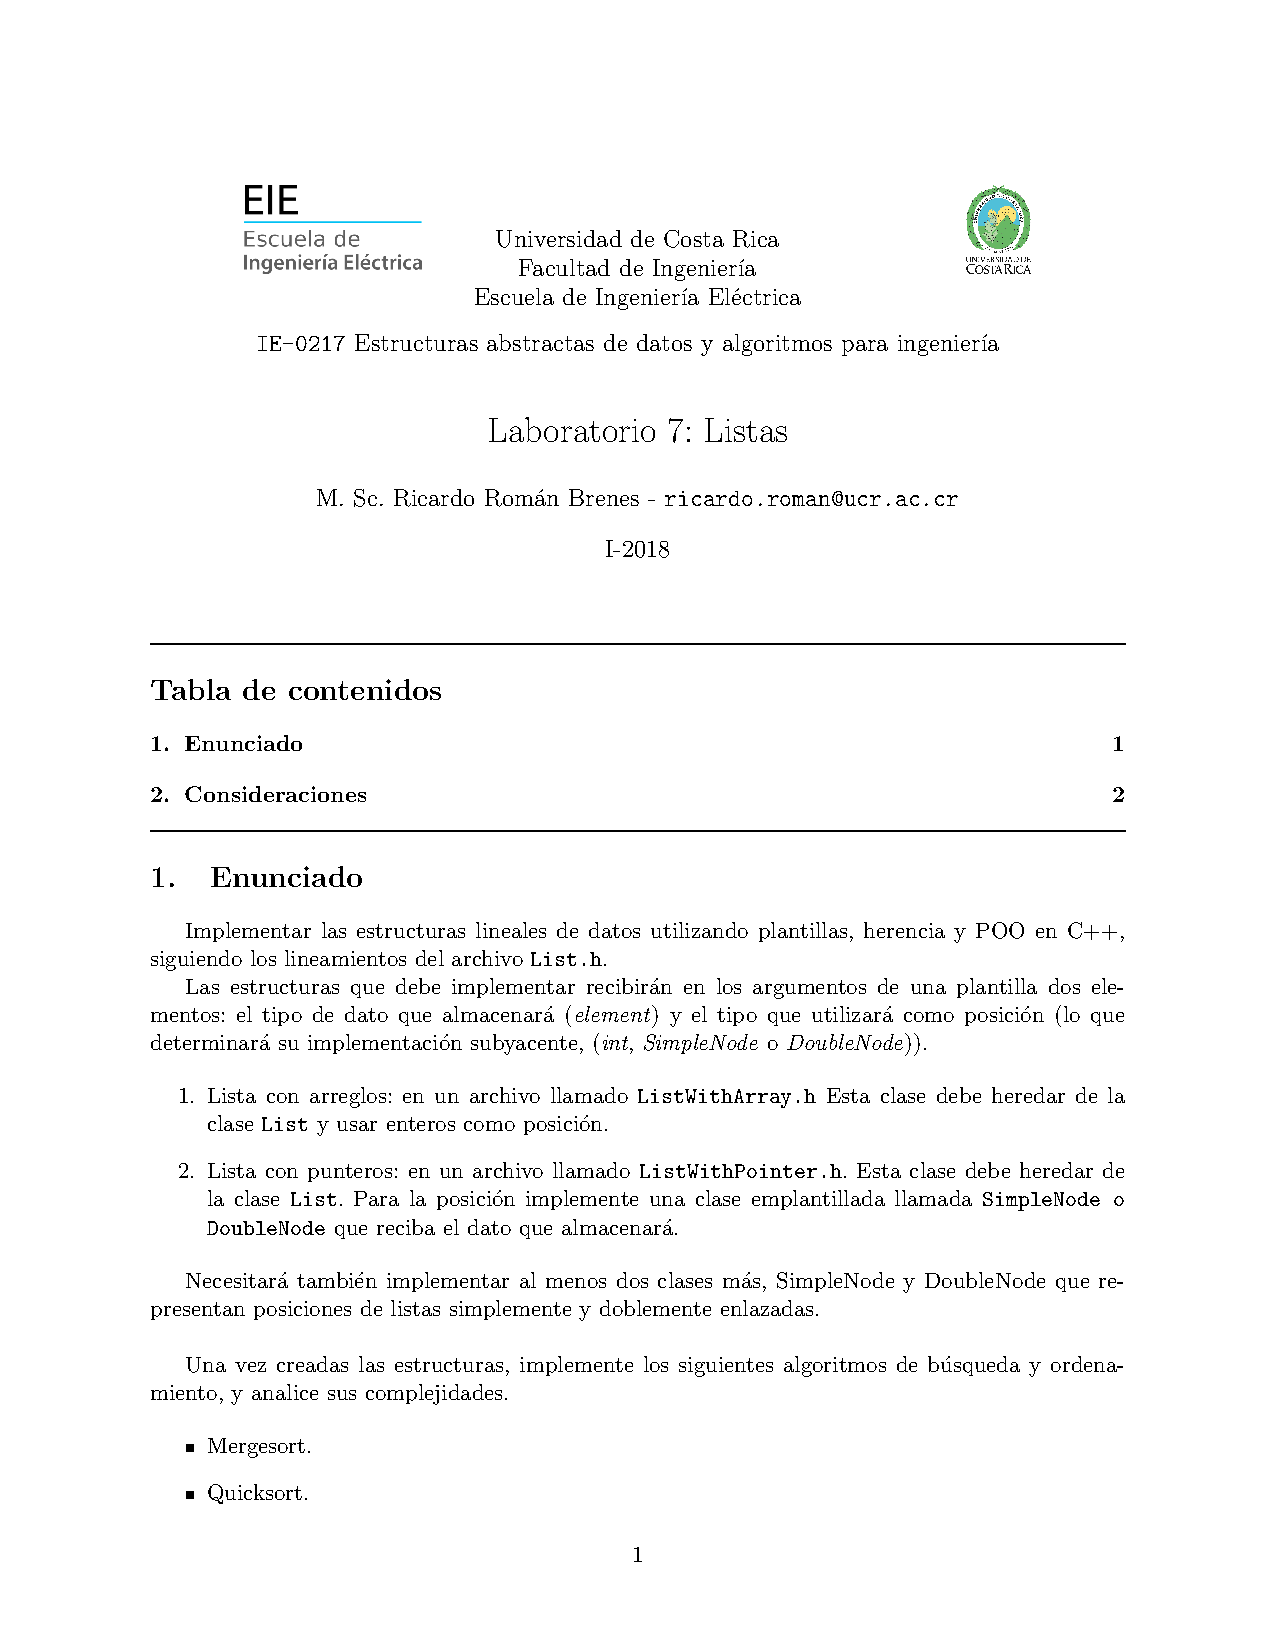
\includepdf[pages=1,pagecommand=\section{Enunciado}, scale=0.8]{enunciados/enun7} 
\includepdf[pages=2,pagecommand={},scale=0.8]{enunciados/enun7}

%%%%%%%%%%%%%%%%%%%%%%%%%%%%%%%%%%%%%%%%%%%%%%%%%%%%%%%%%%%%%%
% --> SOLUCIÓN
%%%%%%%%%%%%%%%%%%%%%%%%%%%%%%%%%%%%%%%%%%%%%%%%%%%%%%%%%%%%%%
\section{Solución}


%------------------------------
\subsection{Lista}
%------------------------------

Esta es la clase base y contiene las declaraciones de las funciones básicas que deben contener las listas implementadas. Es una clase emplantillada, de manera que los objetos de esta clase o las subclases se pueden crear con diferentes tipos de datos, sin afectar la implementación de los métodos. Los argumentos de la plantilla son \texttt{element}, para el tipo de dato que se desea almacenar en la lista, y \texttt{position}, para el tipo de dato que indicará la posición de cada elemento dentro de la lista. En esta clase base existe un atributo \texttt{N} que corresponde a la cantidad actual de elementos o nodos que contiene la lista.

\begin{minted}[linenos,autogobble,bgcolor=bg,breaklines,fontsize=\footnotesize ]{c++}
#ifndef LIST_HPP
#define LIST_HPP

#include "simpleNode.hpp"
#include "doubleNode.hpp"
#include <iostream>
using namespace std;

template<typename element, typename position>
class List
{
  public:
    List(){};
    List(int N){};
    List(const List& orig){};
    virtual ~List(){cout << "/* destructor list */" << endl;};
    virtual void insert(element e, position k) = 0;
    virtual void insert(element e) = 0; // default insert
    virtual bool remove(element e) = 0; // by element
    virtual bool remove(position k) = 0; // by position
    virtual position find(element e) = 0; 
    virtual element find(position k) = 0;
    virtual void print() = 0;
    virtual void emptyList() = 0;
    int getSize();
    virtual position next(position k) = 0;
    virtual position next(element e) = 0;
    virtual position prev(position k) = 0;
    virtual position prev(element e) = 0;
    virtual void replace(element e, position k) = 0;
  protected:
    int N;
  private:
};

#endif /* LIST_HPP */
\end{minted}


%------------------------------
\subsection{Lista con arreglos}
%------------------------------
Una de las formas de implementar la lista enlazada es utilizando arreglos. La clase \texttt{ListWithArray} es también un plantilla y hereda de la clase \texttt{List} con el argumento \texttt{element} para el tipo de dato, mientras que la posición es siempre de tipo \texttt{int}. 

En el constructor se crea un arreglo del tipo de dato especificado, y de un tamaño fijo (tamaño 50 para el constructor sin parámetros, o tamaño especificado en el constructor con parámetro). Este atributo (\texttt{arraySize}) no es equivalente al número de elementos en la lista (\texttt{N}), sino que indica la cantidad de espacio en memoria que se asigna, de manera dinámica, al arreglo creado. En caso de que la lista esté llena (se tienen \texttt{N = arraySize} elementos), se llama a un método que crea un nuevo arreglo con el doble de tamaño y copia los datos (luego limpiando el espacio del arreglo anterior), lo cual permite tener más espacio para insertar más elementos. La razón por la que se eligió doblar el tamaño del arreglo, es por simplicidad y para minimizar la cantidad de veces que se debe recurrir a este método.

\begin{minted}[linenos,autogobble,bgcolor=bg,breaklines,fontsize=\footnotesize ]{c++}
#ifndef LISTWITHARRAY_HPP
#define LISTWITHARRAY_HPP

#include "list.hpp"
#include <iostream>
using namespace std;

template<typename element>
class ListWithArray : public List<element, int>
{
  public:
    ListWithArray(){
        this->data = new element[50];
        this->arraySize = 50;
        this->N = 0;
    };
    
    ListWithArray(int size){
        this->arraySize = size;
        this->data = new element[this->arraySize];
        this->N = 0;
    };

    ListWithArray(const ListWithArray& orig){
        this->data = new element[orig.arraySize];
        this->arraySize = orig.arraySize;
        this->N = orig.N;
        for (int i=0; i<this->N; i++){
            this->data[i] = orig.data[i];
		}
    };

    ~ListWithArray()
    {
      for (int i=0; i<this->arraySize; i++){
        this->data[i] = 0x0;
      }
      delete[] this->data;
      cout << "/* destructor listwitharray */" << endl;
    };

    void insert(element e, int k){
		if (k < this->N){
			if (this->N == this->arraySize){ //si la lista "está llena"
				this->doubleArray();
			}
			for ( int i=(this->N)-1; i>=k; i--){
				this->data[i+1] = this->data[i];
			}
			this->data[k] = e;
			this->N++;
		}
		else if (k == this->N){
			this->data[k] = e;
			this->N++;
		}
		else {
			cout << "Posición fuera del rango del arreglo. Elemento no insertado" << endl;
		}
	};

    void insert(element e){
		if (this->N == this->arraySize){ //esto indicaría que el arreglo está lleno
			this->doubleArray();
		}
		this->data[N] = e;
		this->N++;
	};

    bool remove(element e){// by element
		int c = 0;
		for (int i=0; i<this->N; i++){
			if (this->data[i] == e){
				for (int j=i; j<N; j++){
					this->data[j] = this->data[j+1];
				}
				this->data[N-1] = 0x0;
				N--;
				i--;
				c++;
			}
		}
		if (c!=0){
			return true;
		} else return false;
	}

    bool remove(int k){
		if (k<0 || k>= N){
			cout << "Fuera de rango" << endl;
			return false;
		}
		else {
			for (int j=k; j<N; j++){
				this->data[j] = this->data[j+1];
			}
			this->data[N-1] = 0x0;
			N--;
			return true;
		}
	};

    element find(int k){
  		if (k >= N){
  			//throw
  			cout << "Posición fuera del rango" << endl;
  			return element(-1);
  		} else{
  		return this->data[k];
      }
  	};

    int find(element e){
  		for (int i=0; i<this->N; i++){
        if (this->data[i] == e) return i;
      }
      return -1;
  	};

    void print(){
      if (this->N == 0) cout << "#---lista vacía---#" << endl;
  		for (int i= 0; i<this->N; i++){
  			cout << i << ": " << this->data[i] << endl;
  		}
	};

    void emptyList(){ lista
		for (int i = 0; i<this->arraySize; i++){
			this->data[i] = 0x0;
			this->N = 0;
		}
	};

	int next(int k){
		if (k<0 || k>=N){
			cout << "Fuera de rango" << endl;
			return -1;
		}
		else{
			return k+1;
		}
	};

    int next(element e){
		int p = this->find(e);
		if (p==-1){
			cout << "Fuera de rango" << endl;
			return -1;
			}
		return p+1;
	  };

	int prev(int k){
		if (k==0 || k>N){
			cout << "Fuera de rango" << endl;
			return -1;
		}
		else{
			return k-1;
		}
	};

	int prev(element e){
		int p = this->find(e);
		if (p<=0){
			cout << "Fuera de rango" << endl;
			return -1;
		}
    return p-1;
	};

    int getSize(){
        return this->N;
    };

	void replace(element e, int k){
		if (k < this->N){
			this->data[k] = e;
		}
		else {
			cout << "Fuera de rango" << endl;
		}
	};


  protected:
    int arraySize;	//tamaño del arreglo, fijo
    int N;			//número de elementos, debe ser <= arraySize
    element* data;
    
    void doubleArray(){
		element *temp = new element[2*this->arraySize];
		for (int i=0; i<this->arraySize; i++){
			temp[i] = this->data[i];
		}
		delete [] this->data;
		this->arraySize *= 2;
		this->data = new element[this->arraySize];
		for (int i=0; i<this->arraySize; i++){
			this->data[i] = temp[i];
		}
		delete [] temp;
	}
  private:
};




#endif 
\end{minted}

%------------------------------
\subsection{Lista con punteros}
%------------------------------

En el siguiente código se muestra la estructura de una lista con punteros y la implementación de algunas de sus funciones elementales. Para esta parte algo importante a destacar es que se ha agregado adicionalmente una variable tipo \textbf{int} a los nodos tipo Simple y Doble, con el fin de que sirva de referencia para saber la posición en la lista con punteros de un nodo específico. 

\begin{minted}[linenos,autogobble,bgcolor=bg,breaklines,fontsize=\footnotesize ]{c++}
#ifndef LISTWITHPOINTER_HPP
#define LISTWITHPOINTER_HPP

#include "list.hpp"
#include "simpleNode.hpp"
#include "doubleNode.hpp"
#include <typeinfo>
#include <cstdlib>
#include <iostream>
using namespace std;

template<typename element, typename position>
class ListWithPointer : public List<element, position>
{
  public:

    ListWithPointer()
    {
      cout << "/* constructor listwithpointer */" << endl;
      first = NULL;
      last = NULL;
      this->N = 0;
    };

    ListWithPointer(int N)
    {
      for(int i = 0; i<N; i++) insert((element)i);
    };
    ///@brief Destructor de la clase
    ///@details Llama al método emptyList() para eliminar contenidos
    ///@link ListWithPointer @endlink
    ~ListWithPointer()
    {
      cout << "/* destructor listwithpointer */" << endl;
      this->emptyList();
    };

    void insert(element e, SimpleNode<element> k)
    {
      if(k.pos > this->N || k.pos < 0 ) {cout << "La posición ingresada se encuentra fuera de la lista"<<endl; return;}
      this->N++;
      position* temp;
      if(k.pos ==  0)
      {
        if (first == NULL)
        {
          first = new position(0);
          first->value = e;
          first->next = NULL;
        } else
        {
          temp = new position(0);
          temp->value = e;
          temp->next = first;
          first = temp;
        }
      }else
      {
      position* newElement = new position(k.pos);
      newElement->value = e;
      temp = first;
      for(int i = 0; i<k.pos-1; i++) temp = temp->next;
      newElement->next = (temp->next);
      temp->next = newElement;
      }

      last = new position(0);
      temp = first;
      for(int i = 0; i<k.pos+1; i++) temp = temp->next;
      for(int i = k.pos+1; i<this->N; i++) {temp->pos++; last = temp; temp = temp->next;}
    };

    void insert(element e, DoubleNode<element> k)
    {
      if(k.pos > this->N || k.pos < 0 ) {cout << "La posición ingresada se encuentra fuera de la lista"<<endl; return;}
      this->N++;
      position* temp;
      if(k.pos ==  0)
      {
        if (first == NULL)
        {
          first = new position(0);
          first->value = e;
          first->next = NULL;
          first->prev = NULL;
        } else
        {
          temp = new position(0);
          first->prev = temp;
          temp->value = e;
          temp->prev = NULL;
          temp->next = first;
          first = temp;
        }
      }else
      {
        position* newElement = new position(k.pos);
        newElement->value = e;
        temp = first;
        for(int i = 0; i<k.pos-1; i++) temp = temp->next;
        newElement->prev = temp;
        newElement->next = temp->next;
        temp->next = newElement;
        temp = first;
        //for(int i = 0; i<k.pos-2; i++) temp = temp->next;
        temp->prev = newElement;
      }

      temp = first;
      // last = new position();
      for(int i = 0; i<k.pos+1; i++) temp = temp->next;
      for(int i = k.pos+1; i<this->N; i++)
      {
        temp->pos++;
        //if(i == this->N-2) last = temp;
        temp = temp->next;
      }
      last = new position();
      temp = first;
      for(int i = 0; i<this->N-1; i++) temp = temp->next;
      last = temp;
    };

    void insert(element e)
    {
      this->insert(e,position(this->N));
    };

    bool remove(element e)
    {
      position k = this->find(e);
      if (k.pos == -1) return false;
      this->remove(k);
      return true;
    }; // by element

    bool remove(SimpleNode<element> k)
    {
      if(k.pos > this->N || k.pos < 0 ) {cout << "La posición ingresada se encuentra fuera de la lista"<<endl; return false;}

      position* list = first;
      position* temp  = NULL;

      if (k.pos == 0)
      {
        temp =first->next;
        delete first;
        first = temp;
      }else if(k.pos == this->N-1)
      {
        for (int i = 0; i < k.pos-1; i++) list = list->next;
        temp = list->next;
        list->next = NULL;
        last = list;
        delete temp;
      }else
      {
        for (int i = 0; i < k.pos-1; i++) list = list->next;
        temp = list->next;
        list->next = temp->next;
        delete temp;
      }
      this->N--;
      temp = first;
      for(int i = 0; i<k.pos; i++) temp = temp->next;
      for(int i = k.pos; i<this->N; i++) {temp->pos--; temp = temp->next;}

      temp = first;
      for(int i = 0; i<this->N-1; i++) temp = temp->next;
      last = temp;

      return true;
    }; // by position

    bool remove(DoubleNode<element> k)
    {
      if(k.pos > this->N || k.pos < 0 ) {cout << "La posición ingresada se encuentra fuera de la lista"<<endl; return false;}

      position* list = first;
      position* temp  = NULL;

      if (k.pos == 0)
      {
        temp =first->next;
        temp->prev = NULL;
        delete first;
        first = temp;
      }else if(k.pos == this->N-1)
      {
        for (int i = 0; i < k.pos-1; i++) list = list->next;
        temp = list->next;
        list->next = NULL;
        last = list;
        delete temp;
      }else
      {
        for (int i = 0; i < k.pos-1; i++) list = list->next;
        temp = list->next;
        list->next = temp->next;
        delete temp;
        temp = list->next;
        temp->prev =  list;
      }
      this->N--;
      temp = first;
      for(int i = 0; i<k.pos; i++) temp = temp->next;
      for(int i = k.pos; i<this->N; i++) {temp->pos--; temp = temp->next;}
      return true;
    }; // by position

    position find(element e)
    {
      position* temp = first;
      //--> SOLO RETORNA EL PRIMER ELEMENTO IGUAL QUE SE ENCUENTRA EN LA LISTA
      for(int i = 0; i<this->N; i++)
      {
        if(temp->value == e ) return *temp;
        temp = temp->next;
      }
      cout << "No se encontro el elemento: "<<  e << endl;
      return position(-1);
    };

    element find(position k)
    {
      if(k.pos > this->N || k.pos < 0 ) {cout << "La posición ingresada se encuentra fuera de la lista"<<endl; return element(-1);}
      position* temp = first;
      for(int i = 0; i<k.pos; i++) temp = temp->next;
      return temp->value;
    };

    void sort()
    {
      this->quicksort(0,this->N-1);
    }; // some kind of sorting

    void print()
    {
      if(first->next == NULL) cout << "La lista no tiene elementos"<<endl;
      position* temp = first;
      for (int i =0; i<this->N; i++) {cout << temp->pos << " : " << temp->value << endl; temp = temp->next;}
      //position* temp = last;
      //for (int i =0; i<this->N; i++) {cout << temp->pos << " : " << temp->value << endl; temp = temp->prev;}
    };

    void emptyList()
    {
      this->N = 0;
      position* list;
      position* temp;
      if(first != NULL)
      {
      list = first->next;
      first->next = NULL;
        while(list != NULL)
        {
         temp = list->next;
         delete list;
         list = temp;
        }
      }
    };

    int getSize()
    {
      return this->N;
    };

    position next(position k)
    {
      if(k.pos > this->N || k.pos < 0 ) {cout << "La posición ingresada se encuentra fuera de la lista"<<endl; return position(-1);}
      if(k.pos == this->N-1 ) {cout << "No hay siguiente posición porque es el último elemento de la lista"<< endl; return position(-1);}
      position* temp = first;
      for(int i = 0; i<k.pos; i++) temp = temp->next;
      return *temp->next;
    };

    position next(element e)
    {
      position* temp = first;
      for(int i = 0; i<this->N; i++)
      {
        if(temp->value == e )
        {
          if(i == this->N-1) {cout << "No hay siguiente elemento porque "<<  e <<" es el último de la lista"<< endl; return position(-1);}
          return *temp->next;
        }
        temp = temp->next;
      }
      cout << "No se encontro el elemento: "<<  e << endl;
      return position(-1);
    };

    position prev(SimpleNode<element> k)
    {
      if(k.pos > this->N-1 || k.pos < 0 ) {cout << "La posición ingresada se encuentra fuera de la lista"<<endl; return position(-1);}
      if(k.pos == 0 ) {cout << "No hay posición previa porque es el primer elemento de la lista"<< endl; return position(-1);}

      position* temp = first;
      for(int i = 0; i<k.pos-1; i++) temp = temp->next;
      return *temp;
    };

    position prev(DoubleNode<element> k)
    {
      if(k.pos > this->N-1 || k.pos < 0 ) {cout << "La posición ingresada se encuentra fuera de la lista"<<endl; return position(-1);}
      if(k.pos == 0 ) {cout << "No hay posición previa porque es el primer elemento de la lista"<< endl; return position(-1);}

      position* temp = first;
      for(int i = 0; i<k.pos; i++) temp = temp->next;
      return *temp->prev;
    };

    position prev(element e)
    {
      position k = this->find(e);
      if (k.pos == -1) return position(-1);
      if(k.pos == 0 ) {cout << "No hay posición previa porque " << e <<" es el primer elemento de la lista"<< endl; return position(-1);}

      position* temp = first;
      for(int i = 0; i<k.pos-1; i++) temp = temp->next;
      return *temp;
    };

    void replace(element e, position k)
    {
      if(k.pos > this->N || k.pos < 0 ) {cout << "La posición ingresada se encuentra fuera de la lista"<<endl; return;}
      position* temp = first;
      for(int i = 0; i<k.pos; i++) temp = temp->next;
      temp->value = e;
    };

    void merge(DoubleNode<element> in, DoubleNode<element> c, DoubleNode<element> f)
    {
      position i=in;
      position j=c+1;
      ListWithPointer<element,DoubleNode<element> >* temp = new ListWithPointer<element,DoubleNode<element> >(f.pos-in.pos+1);
      position k=0;
      //
      while ((i<=c) &&(j<=f))
      {
          if(find(i)<find(j))
          {
              temp->replace(find(i),k);
              i++;
          }
          else
          {
              temp->replace(find(j),k);
              j++;
          }
          k++;
      }
      while (i<=c)
      {
          temp->replace(find(i),k);
          i++;
          k++;
      }
      while (j<=f)
      {
          temp->replace(find(j),k);
          j++;
          k++;
      }
      //temp->print();
      //cout << k.pos << '\n';
      for(i=0;i<k;i++)
      {
          //cout << temp->find(i) << '\n';
          this->replace(temp->find(i),i+in);
      }
      temp->~ListWithPointer();
    };
    
    void merge(SimpleNode<element> in, SimpleNode<element> c, SimpleNode<element> f)
    {
      position i=in;
      position j=c+1;
      ListWithPointer<element,SimpleNode<element> >* temp = new ListWithPointer<element,SimpleNode<element> >(f.pos-in.pos+1);
      position k=0;
      //
      while ((i<=c) &&(j<=f))
      {
          if(find(i)<find(j))
          {
              temp->replace(find(i),k);
              i++;
          }
          else
          {
              temp->replace(find(j),k);
              j++;
          }
          k++;
      }
      while (i<=c)
      {
          temp->replace(find(i),k);
          i++;
          k++;
      }
      while (j<=f)
      {
          temp->replace(find(j),k);
          j++;
          k++;
      }
      //temp->print();
       //cout << k.pos << '\n';
      for(i=0;i<k;i++)
      {
          //cout << temp->find(i) << '\n';
          this->replace(temp->find(i),i+in);
      }
      temp->~ListWithPointer();
    };
  protected:
    position* first;
    position* last;
  private:
};

#endif /* LISTWITHPOINTER_HPP */
\end{minted}

%------------------------------
\subsubsection{Lista Simple}
%------------------------------
Una lista enlazada es una de las estructuras de datos fundamentales, y puede ser usada para implementar otras estructuras de datos. Consiste en una secuencia de nodos, en los que se guardan campos de datos arbitrarios y una o dos referencias, enlaces o punteros al nodo anterior o posterior. En la figura \ref{fig:LES} se muestra la estructura típica de una lista enlazada simple.

\begin{figure}[H]
\centering
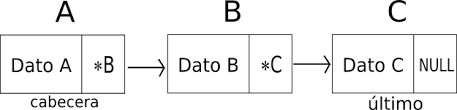
\includegraphics[width=0.55\textwidth]{imgs/Labo7/simp.png}
\caption{Lista Enlazada Simple}
\label{fig:LES}
\end{figure}

A continuación se describe el código desarrollado para crear un clase que describa un nodo de este tipo de datos.

\begin{minted}[linenos,autogobble,bgcolor=bg,breaklines,fontsize=\footnotesize ]{c++}
#ifndef SIMPLENODE_HPP
#define SIMPLENODE_HPP

#include <iostream>

template<typename element>
class SimpleNode
{
  public:
    SimpleNode(){};
    SimpleNode(int k)
    {
      this->pos = k;
      this->value = element(NULL);
      this->next = NULL;
    };
    SimpleNode(const SimpleNode<element> &copy)
    {
      this->pos = copy.pos;
      this->value = copy.value;
      this->next = copy.next;
    };
    //------------------------------------------------------------------------//
    element       value;
    SimpleNode*   next;
    int  pos;
    //-----------------------Sobrecarga de Operadores-------------------------//
    SimpleNode operator+(int k)
    {
      return SimpleNode(this->pos+k);
    };
    SimpleNode operator+(SimpleNode k)
    {
      return SimpleNode(this->pos+k.pos);
    };
    SimpleNode operator/(int k)
    {
      return SimpleNode((int)this->pos/k);
    };
    SimpleNode operator/(SimpleNode k)
    {
      return SimpleNode((int)this->pos/k.pos);
    };
    SimpleNode operator++(int)
    {
      return SimpleNode(this->pos++);
    };
    SimpleNode operator-(int k)
    {
      return SimpleNode(this->pos-k);
    };
    SimpleNode operator-(SimpleNode k)
    {
      return SimpleNode(this->pos-k.pos);
    };
    SimpleNode operator--(int)
    {
      return SimpleNode(this->pos++);
    };
    SimpleNode operator=(int k)
    {
      return SimpleNode(k);
    };
    bool operator==(SimpleNode k)
    {
      if(this->pos==k.pos) return true;
      else return false;
    };
    bool operator<(SimpleNode k)
    {
      if(this->pos<k.pos) return true;
      else return false;
    };
    bool operator>(SimpleNode k)
    {
      if(this->pos>k.pos) return true;
      else return false;
    };
    bool operator<=(SimpleNode k)
    {
      if(this->pos<=k.pos) return true;
      else return false;
    };
    bool operator>=(SimpleNode k)
    {
      if(this->pos>=k.pos) return true;
      else return false;
    };
  protected:
  private:
};

#endif /* SIMPLENODE_HPP */
\end{minted}

%------------------------------
\subsubsection{Lista Doble}
%------------------------------

La lista doblemente enlazada es una estructura de datos que consiste en un conjunto de nodos enlazados secuencialmente. Cada nodo contiene dos campos, llamados enlaces, que son referencias al nodo siguiente y al anterior en la secuencia de nodos. El enlace al nodo anterior del primer nodo y el enlace al nodo siguiente del último nudo, apuntan a un tipo de nodo que marca el final de la lista, normalmente un puntero null,para facilitar el recorrido de la lista. Este tipo de estructuta se puede observar en la figura \ref{fig:LDE}.

\begin{figure}[H]
\centering
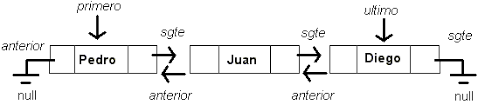
\includegraphics[width=0.7\textwidth]{imgs/Labo7/dob.png}
\caption{Lista Doblemente Enlazada}
\label{fig:LDE}
\end{figure}

A continuación se describe el código desarrollado para crear un clase que describa un nodo de este tipo de datos.

\begin{minted}[linenos,autogobble,bgcolor=bg,breaklines,fontsize=\footnotesize ]{c++}
#ifndef DOUBLENODE_HPP
#define DOUBLENODE_HPP

#include <iostream>
using namespace std;


template<typename element>
class DoubleNode
{
  public:
    DoubleNode(){};
    DoubleNode(int k)
    {
      this->pos = k;
      this->value = element(NULL);
      this->next = NULL;
      this->prev = NULL;
    };
    DoubleNode(const DoubleNode<element> &copy)
    {
      this->pos = copy.pos;
      this->value = copy.value;
      this->next = copy.next;
      this->prev = copy.prev;
    };
    //------------------------------------------------------------------------//
    element     value;
    DoubleNode* next;
    DoubleNode* prev;
    int  pos;
    //-----------------------Sobrecarga de Operadores-------------------------//
    DoubleNode operator+(int k)
    {
      return DoubleNode(this->pos+k);
    };
    DoubleNode operator+(DoubleNode k)
    {
      return DoubleNode(this->pos+k.pos);
    };
    DoubleNode operator/(int k)
    {
      return DoubleNode(((int)this->pos)/k);
    };
    DoubleNode operator/(DoubleNode k)
    {
      return DoubleNode((int)this->pos/k.pos);
    };
    DoubleNode operator++(int)
    {
      return DoubleNode(this->pos++);
    };
    DoubleNode operator-(int k)
    {
      return DoubleNode(this->pos-k);
    };
    DoubleNode operator-(DoubleNode k)
    {
      return DoubleNode(this->pos-k.pos);
    };
    DoubleNode operator--(int)
    {
      return DoubleNode(this->pos++);
    };
    DoubleNode operator=(int k)
    {
      return DoubleNode(k);
    };
    bool operator==(DoubleNode k)
    {
      if(this->pos == k.pos){return true;}
      else {return false;}
    };
    bool operator<(DoubleNode k)
    {
      if(this->pos<k.pos) return true;
      else return false;
    };
    bool operator>(DoubleNode k)
    {
      if(this->pos>k.pos) return true;
      else return false;
    };
    bool operator<=(DoubleNode k)
    {
      if(this->pos<=k.pos) return true;
      else return false;
    };
    bool operator>=(DoubleNode k)
    {
      if(this->pos>=k.pos) return true;
      else return false;
    };
  protected:
  private:
};

#endif /* DOUBLENODE_HPP */
\end{minted}

%------------------------------
\subsection{Algoritmos de búsqueda y ordenamiento}
%------------------------------

%------------------------------
\subsubsection{Mergesort}
%------------------------------

El algoritmo de \texttt{mergesort} consiste en un algoritmo del tipo \textit{divide y vencerás}. Este algoritmo toma una lista y la divide en dos del mismo tamaño, y se llama recursivamente para cada mitad de la lista. Esto lo realiza hasta que queda la lista original dividida en pequeñas listas que contienen solo un elemento, en este momento compara los valores de ellas y los ordena, donde luego procede a ir uniendo los segmentos, hasta obtener una única lista ordenada. Se sabe que este algoritmo tiene un tiempo de ejecución de la forma\cite{R3}:
\begin{equation}
    T(n)=\left\lbrace
\begin{array}{ll}
 O(1) & n=1\\
 2T(n/2)+O(n) & n>1
\end{array}
\right.
\end{equation}
Donde aplicando el teorema maestro se observa que $a=2$, $b=2$ y por lo tando $d=1$. Entonces se sabe que este algoritmo tiene una complejidad $O(n\log{n})$. 

%------------------------------
\subsubsection{Quicksort}
%------------------------------
Al igual que el algoritmo \texttt{mergesort}, \texttt{quicksort} consiste en un algoritmo del tipo \textit{divide y vencerás}. Este algoritmo toma un valor de la lista (en este caso el último) como pivote y ordena a un lado de él todos los elementos menores, y al otro lado los elementos mayores. De esta forma el pivote queda justamente en la posición que le corresponde y la lista se divide en dos sublistas a las cuales se les aplica nuevamente el algoritmo, hasta que queden listas de únicamente un elemento, es decir, cuando la lista esté ordenada. Este algoritmo presenta un tiempo de ejecución igual al caso del \texttt{mergesort}, lo que se traduce en una complejidad $O(n\log n)$, pero esta es la complejidad del caso promedio. Si se presenta la situación de que la lista esté ordenada o casi ordenada, se presenta el peor de los caso debido a que tiene que recorrer toda la lista, en esta situación la complejidad crece a $O(n^2)$\cite{R3}.  

Para implementar este algoritmo en el código de C++, se crearon dos funciones, una propiamente del algoritmo, \texttt{quicksort}, y otra función auxiliar \texttt{partition} encargada de realizar la partición para ejecutar el algoritmo de forma recursiva.

\begin{minted}[linenos,autogobble,bgcolor=bg,breaklines,fontsize=\footnotesize ]{c++}
    position partition(position l, position r)
    {
      element pivote = find(r);
      position i = l-1;
      for(position k = l; k < r; k++)
      {
        if( find(k) <= pivote )
        {
          i++;
          swap(i,k);
        }
      }
      swap(i+1,r);
      return(i+1);
    };
    void quicksort(position l,position r)
    {
      if(l < r)
      {
        position m = partition(l,r);
        quicksort(l, m-1);
        quicksort(m+1,r);
      }
    };
\end{minted}

%------------------------------
\subsubsection{Selection Sort}
%------------------------------

Este algoritmo recorre la lista buscando el elemento con el menor valor, una vez que lo encuentra lo posiciona en la primera posición y vuelve a realizar lo mismo para la lista omitiendo el valor recién acomodado, de esta forma la lista se va reduciendo hasta que queda un solo elemento y la lista se encuentra ordenada. Este algoritmo requiere de dos ciclos \texttt{for} anidados para ejecutarse, por lo tanto posee una complejidad $O(n^2)$. 
\begin{minted}[linenos,autogobble,bgcolor=bg,breaklines,fontsize=\footnotesize ]{c++}
void selectionsort(position n)
    {
      position min;
      for(position i = 0; i <n-1; i++)
      {
        min = i;
        for(position j = i+1; j<n; j++)
        {
          if( find(j) < find(min) )
          {
            min = j;
          }
        }
        swap(min, i);
      }
    };
\end{minted}

Es importante mencionar que tanto \texttt{Selection Sort} como \texttt{Quicksort} requieren implementar una función \texttt{swap} que intercambie la posición de dos elementos de la lista. Esto se logra implementando esta función en \texttt{list.hpp}, así como una función \texttt{replace(element e, position k)} que reemplaza el elemento \texttt{e} en la posición \texttt{k}.

\begin{minted}[linenos,autogobble,bgcolor=bg,breaklines,fontsize=\footnotesize ]{c++}
virtual void swap(position a, position b){
      element temp = find(a);
      replace(find(b), a );
      replace(temp, b );
};
\end{minted}





%------------------------------
\subsubsection{Búsqueda lineal}
%------------------------------
La búsqueda lineal es el algoritmo más intuitivo a la hora de buscar un elemento en la lista. Este algoritmo consiste en simplemente recorrer toda la lista elemento por elemento hasta encontrar el elemento deseado. Esta función depende únicamente del largo $n$ de la lista, por lo tanto tiene una complejidad O(n). La función implementada recibe como argumentos el elemento que se desea buscar, seguido por el tamaño de la lista.

\begin{minted}[linenos,autogobble,bgcolor=bg,breaklines,fontsize=\footnotesize ]{c++}
position linealsearch(element e, position k)
    {
      for(position i=0; i < k ; i++)
      {
        if( find(i) == e ){ return i; }
      }
      return -1;
    };
\end{minted}

%------------------------------
\subsubsection{Búsqueda binaria}
%------------------------------
La búsqueda binaria toma una lista ordenada y la divide en dos, luego se procede a comparar el valor del elemento en la mitad de la lista y dependiendo de si este es mayor o menor se realiza nuevamente la búsqueda en la mitad correspondiente. Si el elemento en la mitad de la lista corresponde al elemento buscado, se devuelve la posición y se termina la búsqueda. Este algoritmo depende de la cantidad de veces que se puede dividir la lista de largo $n$ entre $2$ hasta que se tenga un $1$, por esto se tiene que $1=n/2^x$. Despejando la expresión se obtiene que $x=\log_2 n$, entonces la complejidad del algoritmo corresponde a $O(\log n)$\cite{R3}, lo cual es mejor que la búsqueda lineal.

En este caso el algoritmo recibe las posiciones inicial y final de la lista, así como el elemento que se desea buscar.

\begin{minted}[linenos,autogobble,bgcolor=bg,breaklines,fontsize=\footnotesize ]{c++}
position binarysearch(position l, position r, element e)
    {
      if( r>=1 )
      {
        position mitad = l + (r-l)/2;
        if( find(mitad)==e ) return mitad;
        else if ( find(mitad) > e ){return binarysearch(l, mitad-1, e);}
        else return binarysearch(mitad+1, r, e);
      }
      return -1;
    };
\end{minted}

%------------------------------
\subsubsection{Búsqueda Fibonacci}
%------------------------------
Este algoritmo de búsqueda requiere de una lista ordenada, y es del tipo \textit{divide y vencerás}.Su funcionamiento es similar al de la búsqueda binaria, pero en lugar de dividir la lista entre dos, utiliza los números de la secuencia de Fibonacci. En su funcionamiento, el algoritmo primero encuentra el menor número de la secuencia de Fibonacci que sea mayor o igual al tamaño de la lista, con el fin de utilizarlo de límite para la iteración. Una vez que se sabe esto, el algoritmo obtiene un valor que utiliza como punto de comparación y compara si el valor de la lista en este punto es menor, igual o mayor al elemento buscado, y así delimita la búsqueda. Con ayuda de una variable denominada \texttt{offset} se desprecian los valores a la izquierda de la lista en cierto intervalo, y así se va reduciendo cada vez más la búsqueda hasta obtener el valor deseado. Al igual que en el algoritmo de búsqueda binaria, este algoritmo presenta una complejidad del orden $O(\log n)$.

\begin{minted}[linenos,autogobble,bgcolor=bg,breaklines,fontsize=\footnotesize ]{c++}
    position fibonaccisearch(element e, position n){
      position m = 0;
      while (generadorFibonacci(m) < n ) {
        m = m+1;
      }
      cout << "Posicion de Fibonacci a utilizar: " << m.pos << endl;
      position offset = -1;
      while (generadorFibonacci(m)>1) {
        position i = minimum( offset+generadorFibonacci(m-2) , n-1 );
        if (e > find(i) ) {
          m = m-1;
          offset = i;
        }
        else if(e < find(i)){
          m = m-2;
        }
        else {return i;}
      }
      if(generadorFibonacci(m)<=1){
        if(find(offset+1)==e){
          return offset+1;
        }
      }
      return -1;
    };
\end{minted}

Para que este algoritmo funcione en nuestro código, es necesario programar dos funciones auxiliares \texttt{generadorFibonacci} y \texttt{minimum}. La primera de estas, como su nombre lo menciona, genera el n-ésimo número de la secuencia de Fibonacci. La función \texttt{minimum} compara el valor de dos elementos, y retorna el de menor tamaño.

\begin{minted}[linenos,autogobble,bgcolor=bg,breaklines,fontsize=\footnotesize ]{c++}
    position generadorFibonacci(position n){
      if(n<1){return 0;}
      else if(n==1){return 1;}
      else {
        return generadorFibonacci(n-1)+generadorFibonacci(n-2);
      }
    };
    position minimum(position a, position b){
      if(a <= b){ return a; }
      else { return b; }
    }
\end{minted}

%%%%%%%%%%%%%%%%%%%%%%%%%%%%%%%%%%%%%%%%%%%%%%%%%%%%%%%%%%%%%%
% --> RESULTADOS
%%%%%%%%%%%%%%%%%%%%%%%%%%%%%%%%%%%%%%%%%%%%%%%%%%%%%%%%%%%%%%
\section{Resultados}

Se realizó un programa principal con el fin de probar el funcionamiento de las clases creadas, en el cual se crean instancias de cada tipo de lista y se ejecutan algunos de sus métodos. 

\begin{minted}[linenos,autogobble,bgcolor=bg,breaklines,fontsize=\footnotesize ]{c++}
#include <cstdlib>
#include <iostream>

#include "../include/list.hpp"
#include "../include/listWithArray.hpp"
#include "../include/listWithPointer.hpp"

using namespace std;

int main(int argc, char** argv)
{
...
}
\end{minted}

\subsection{Validación lista con arreglo}

Para probar la lista con arreglos, se crea un objeto del tipo ListWithArray, el cual se inicializa con un tamaño de 7. Si se imprime la lista recién creada, sin elementos, se imprime el mensaje "lista vacía". Conforme se agregan elementos, si se excede el tamaño del arreglo inicialmente asignado, éste doblará su tamaño automáticamente para permitir seguir insertando elementos, de modo que nunca se tendrá una "lista llena". En este ejemplo se ejecutan los métodos \texttt{insert, remove, find, next, prev, getSize} y además se observa el ordenamiento de la lista con \texttt{quicksort} y \texttt{selectionsort}. 

\begin{minted}[linenos,autogobble,bgcolor=bg,breaklines,fontsize=\footnotesize ]{c++}
cout << "Creando lista con array de tamaño 7" << endl;
List<double,int>* l2 = new ListWithArray<double>(7);
l2->print();
cout << "Agregando elementos" << endl;
l2->insert(17.45);
for (int i=1; i<10; i++){
    l2->insert((double)(i*i*0.957-i*4.5));
}
for (int i=7; i<11; i++){
    l2->insert(17.45, i);
}
l2->print();
cout << "Borrando todos los 17.45" << endl;
l2->remove(17.45);
l2->insert(4.44,6);
l2->print();
int tam1 = l2->getSize();
cout << "Tamaño: " << tam1 << endl;
cout << "Encontrando elemento en posición 5: " << l2->find(5) << endl;
cout << "Encontrando posición del elemento 4.44: " << l2->find(4.44) << endl;
cout << "Encontrando posición previa a la del elemento 4.44: " << l2->prev(4.44) << endl;
cout << "Encontrando posición siguiente a la delete elemento 4.44: " << l2->next(4.44) << endl;
cout << "Probando selection sort" << endl;
l2->selectionsort(l2->getSize());
l2->print();
for (int i=0; i<5;i++){
    l2->insert(3.3,i*2);
}
cout << "Lista desordenada" << endl;
l2->print();
cout << "Probando quick sort" << endl;
l2->quicksort(0,l2->getSize()-1);
l2->print();
\end{minted}

De la ejecución del código anterior se obtiene el resultado mostrado en la figura \ref{F:res_list_arr}.

\begin{figure}[H]
\centering
\begin{tabular}{c c}
\subfloat[]{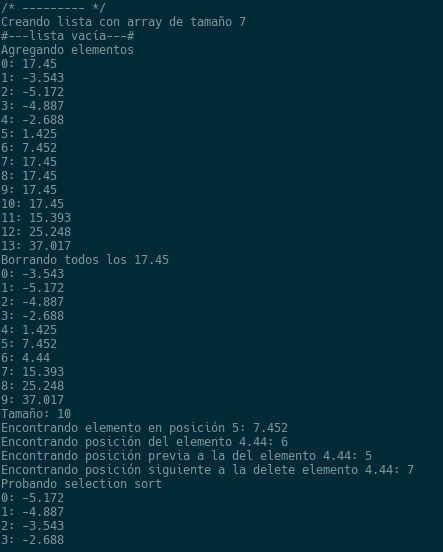
\includegraphics[width=0.52\textwidth]{imgs/Labo7/res1}}    &
\subfloat[]{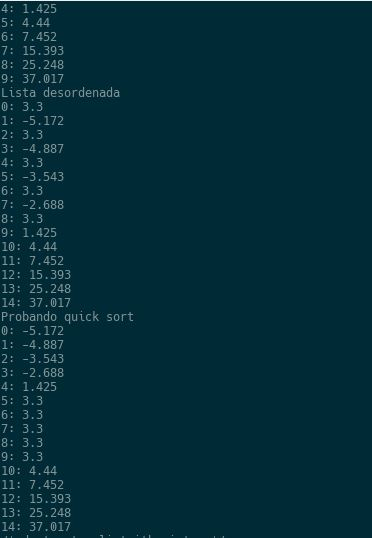
\includegraphics[width=0.45\textwidth]{imgs/Labo7/res2}}    \\
\end{tabular}
\caption{Prueba de la lista con arreglos}
\label{F:res_list_arr}
\end{figure}

\subsection{Validación lista enlazada simple}

Para probar el funcionamiento de la lista con puntero con nodo simple, se crea una instancia de la clase respectiva especificando el tipo de dato que se desea guardar: \texttt{ListWithPointer<double, SimpleNode<double> >}.

\begin{minted}[linenos,autogobble,bgcolor=bg,breaklines,fontsize=\footnotesize ]{c++}
ListWithPointer<double, SimpleNode<double> >* l1 = new ListWithPointer<double, SimpleNode<double> >();
  cout << "/* --------- */" << '\n';
  std::cout << "CREANDO LA LISTA Y ANADIENDO ELEMENTOS" << '\n';
  l1->insert(-0.7);
  l1->insert(0.8);
  l1->insert(-7.7,SimpleNode<double>(1));
  l1->insert(9.9934);
  l1->insert(5.7435);
  l1->insert(35.345);
  l1->insert(2.7);
  l1->insert(-7.7);
  l1->insert(31.7);
  l1->insert(2.7,SimpleNode<double>(0));
  l1->insert(44.7,SimpleNode<double>(6));
  l1->print();
  cout << "/* --------- */" << '\n';
  cout << "Borrando elemento 31.7" << endl;
  l1->remove(31.7);
  l1->print();
  cout << "Borrando elemento en la posición 6" << endl;
  l1->remove(SimpleNode<double>(6));
  l1->print();
  cout << "Encontrando elemento en posición 5: " << l1->find(SimpleNode<double>(5)) << endl;
  cout << "Encontrando posición del elemento 44.7: " << l1->find(44.7).pos << endl;
  cout << "Encontrando posición previa a la del elemento 9.9934: " << l1->prev(9.9934).pos << endl;
  cout << "Encontrando posición siguiente a la del elemento 0.8: " << l1->next(0.8).pos << endl;
  cout << "Tamaño de la lista: " << l1->getSize() << endl;
  delete l1;
\end{minted}
Con el código anterior se obtiene la salida mostrada en la figura \ref{F:res_list_punt_simp}.

\begin{figure}[H]
\centering
\begin{tabular}{c c}
\subfloat[]{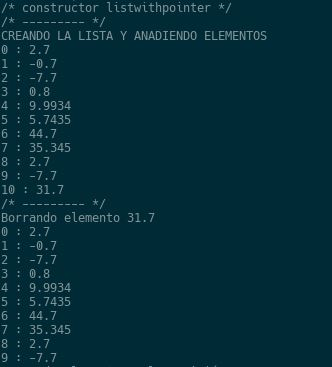
\includegraphics[width=0.43\textwidth]{imgs/Labo7/res3}}    &
\subfloat[]{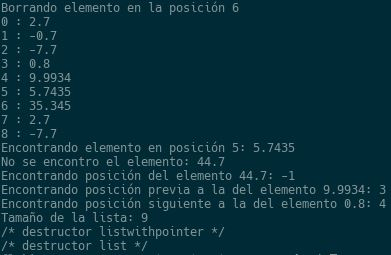
\includegraphics[width=0.55\textwidth]{imgs/Labo7/res4}}    \\
\end{tabular}
\caption{Prueba de la lista puntero, nodo doble}
\label{F:res_list_punt_simp}
\end{figure}

\subsection{Validación lista enlazada doble}
Igual que en el caso anterior, se crea un elemento del tipo de lista especificando el tipo de dato a utilizar: \texttt{ListWithPointer<double, DoubleNode<double> >}. 


\begin{minted}[linenos,autogobble,bgcolor=bg,breaklines,fontsize=\footnotesize ]{c++}
ListWithPointer<double, DoubleNode<double> >* l1 = new ListWithPointer<double, DoubleNode<double> >();
  cout << "/* --------- */" << '\n';
  std::cout << "CREANDO LA LISTA Y ANADIENDO ELEMENTOS" << '\n';
  l1->insert(0.7);
  l1->insert(6.7);
  l1->insert(1.7);
  l1->insert(5.7);
  l1->insert(-7.7,DoubleNode<double>(1));
  l1->insert(30.7);
  l1->insert(2.7);
  l1->insert(-7.7);
  l1->insert(31.7);
  l1->insert(2.7,DoubleNode<double>(0));
  l1->insert(44.7,DoubleNode<double>(6));
  l1->print();
  cout << "/* --------- */" << '\n';
  cout << "Borrando elemento 5.7" << endl;
  l1->remove(5.7);
  l1->print();
  cout << "Borrando elemento en la posición 6" << endl;
  l1->remove(DoubleNode<double>(6));
  l1->print();
  cout << "Encontrando elemento en posición 5: " << l1->find(DoubleNode<double>(5)) << endl;
  cout << "Encontrando posición del elemento 31.7: " << l1->find(31.7).pos << endl;
  cout << "Encontrando posición previa a la del elemento 6.7: " << l1->prev(6.7).pos << endl;
  cout << "Encontrando posición siguiente a la del elemento 1.7: " << l1->next(1.7).pos << endl;
  cout << "Tamaño de la lista: " << l1->getSize() << endl;
  delete l1;
\end{minted}

Con el código anterior, el resultado obtenido en pantalla se muestra en la figura \ref{F:res_list_punt_dob}:

\begin{figure}[H]
\centering
\begin{tabular}{c c}
\subfloat[]{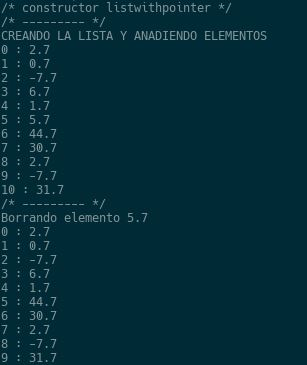
\includegraphics[width=0.43\textwidth]{imgs/Labo7/res5}}    &
\subfloat[]{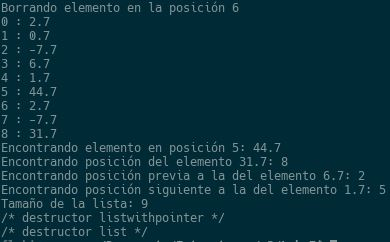
\includegraphics[width=0.55\textwidth]{imgs/Labo7/res6}}    \\
\end{tabular}
\caption{Prueba de la lista puntero, nodo doble}
\label{F:res_list_punt_dob}
\end{figure}


\subsection{Algoritmos de ordenamiento y búsqueda: complejidad y tiempos de ejecución}
A continuación se muestra en las Figuras \ref{fig:slect}, \ref{fig:quick} y \ref{fig:busq} los resultados de ejecutar los algoritmos de búsqueda y ordenamiento. En la Figura \ref{fig:slect} observamos cómo \texttt{selection sort} ordena correctamente la lista, lo mismo sucede en la Figura \ref{fig:quick} para el algoritmo de \texttt{quicksort}. En la Figura \ref{fig:busq} se observa el correcto funcionamiento de los métodos de búsqueda. Es importante notar que la búsqueda lineal se ejecuta sobre una lista desordenada y obtiene un resultado correcto. Luego de esto, es necesario ordenar la lista para que los algoritmos de búsqueda binaria y de Fibonacci funcionen correctamente, en caso de que la lista esté desordenada es muy probable que se genere un error de tipo \textit{segmentation fault}, o que nunca encuentre el elemento buscado.

\begin{figure}[H]
\centering
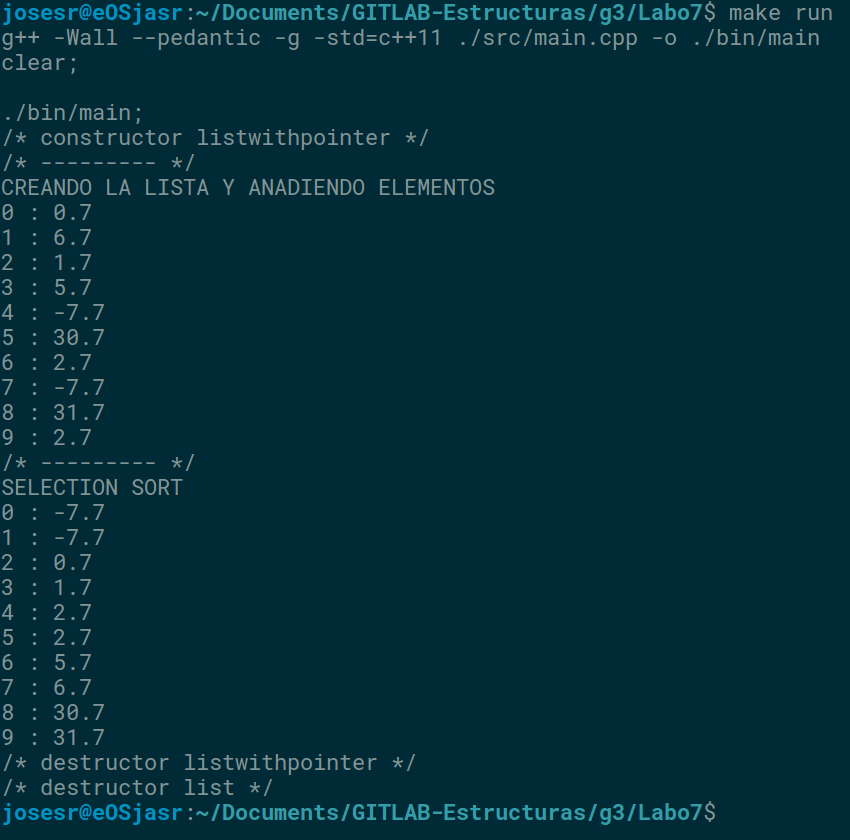
\includegraphics[width=\textwidth]{imgs/Labo7/selection(1).png}
\caption{\texttt{Selection Sort}.}
\label{fig:slect}
\end{figure}

\begin{figure}[H]
\centering
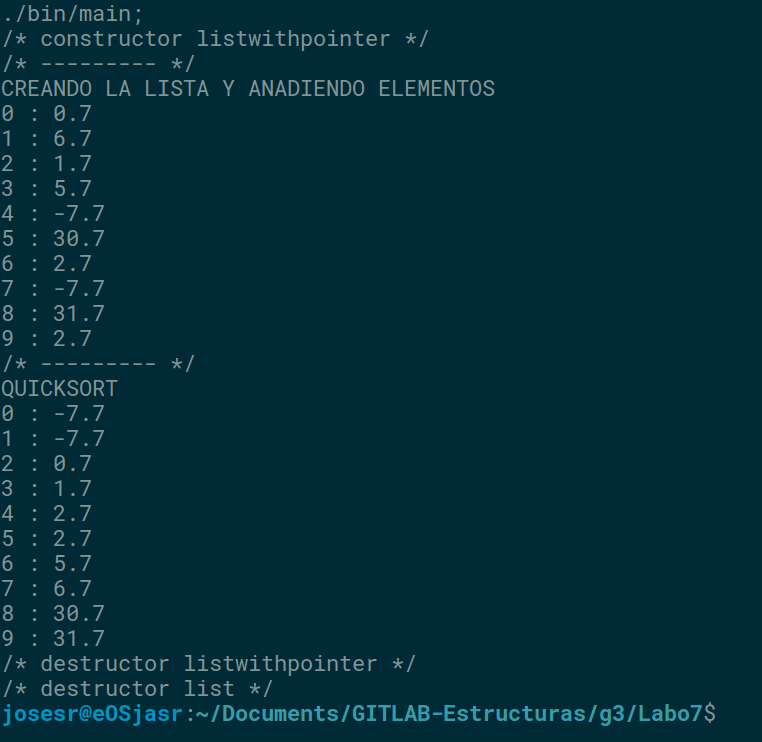
\includegraphics[width=\textwidth]{imgs/Labo7/quick.png}
\caption{\texttt{Quicksort}.}
\label{fig:quick}
\end{figure}

\begin{figure}[H]
\centering
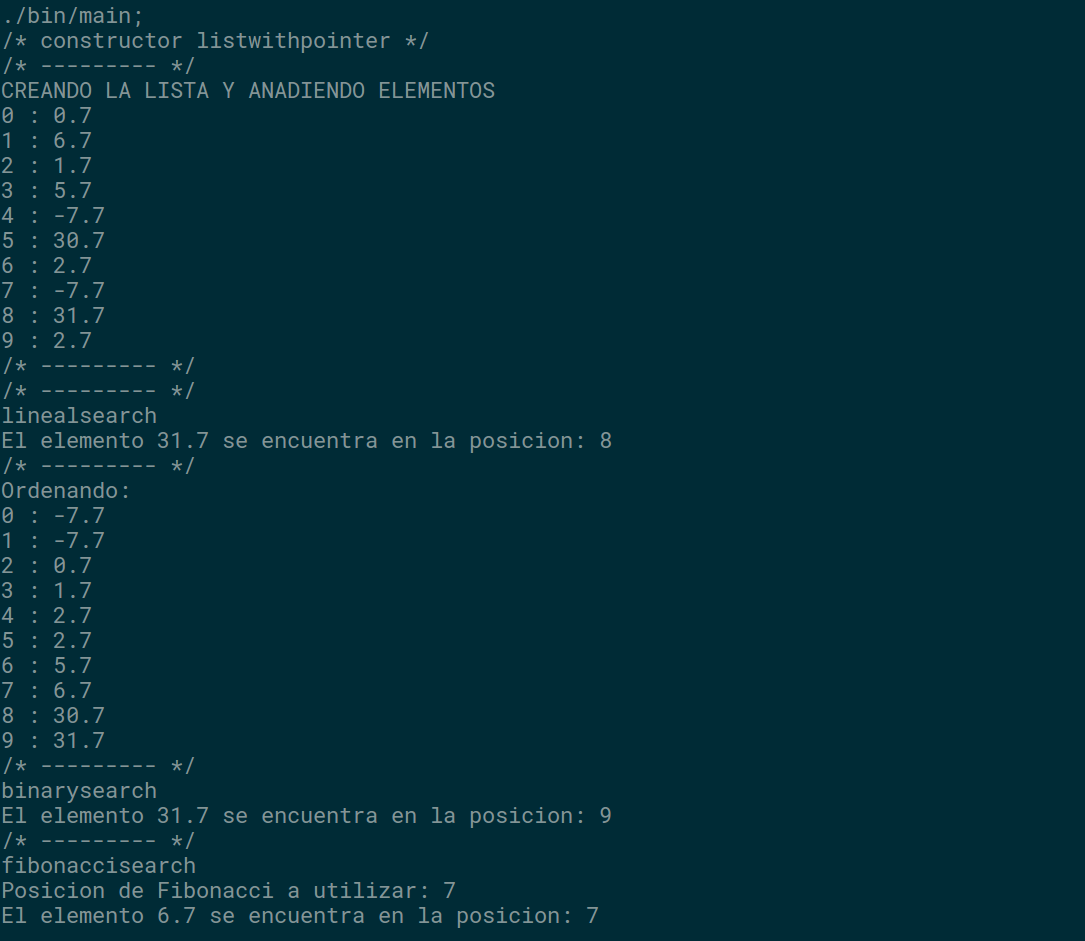
\includegraphics[width=\textwidth]{imgs/Labo7/busq.png}
\caption{Búsqueda de elementos mediante \texttt{linealsearch}, \texttt{binarysearch} y \texttt{fibonaccisearch}.}
\label{fig:busq}
\end{figure}



%%%%%%%%%%%%%%%%%%%%%%%%%%%%%%%%%%%%%%%%%%%%%%%%%%%%%%%%%%%%%%
% --> CONCLUSIONES
%%%%%%%%%%%%%%%%%%%%%%%%%%%%%%%%%%%%%%%%%%%%%%%%%%%%%%%%%%%%%%
\section{Conclusiones}


Como conclusiones se tiene que:

\begin{itemize}
\item Se logró utilizar plantillas y programación orientada a objetos para crear estructuras lineales de tipo lista enlazada, en la que se pueden utilizar diferentes tipos de datos para almacenar los valores y las posiciones.
\item Se implementaron las clases \texttt{DoubleNode} y \texttt{SimpleNode} para utilizarlas como tipos de dato indicadores de posición en la plantilla.
\item Se crearon listas con punteros doblemente enlazadas y simplemente enlazadas, así como listas tipo arreglo. 
\item Se implementaron algoritmos de búsqueda y ordenamiento.

\end{itemize}


%%%%%%%%%%%%%%%%%%%%%%%%%%%%%%%%%%%%%%%%%%%%%%%%%%%%%%%%%%%%%%
% --> BIBLIOGRAFIA
%%%%%%%%%%%%%%%%%%%%%%%%%%%%%%%%%%%%%%%%%%%%%%%%%%%%%%%%%%%%%%
\begin{thebibliography}{IEEE}
\bibitem{R1} Talens, S. \textbf{\textit{Curso de programación en C++}}. EUI (UPV) Valencia, 17 al 28 de Julio de 1995. 

\bibitem{R2} Raffo, E. \textbf{\textit{Programación genérica en C++, usando Metaprogramación}}. 2007. Sistemas de Informática. 

\bibitem{R3} Fillottrani, P. \textbf{\textit{Algoritmos y Complejidad:
Algoritmos “dividir y conquistar”}}. Depto. Ciencias e Ingeniería de la Computación, Universidad Nacional del Sur. Visto el 8 de Junio del 2018 en: \url{http://www.cs.uns.edu.ar/~prf/teaching/AyC17/downloads/Teoria/DividirYConquistr-1x1.pdf} 
\end{thebibliography}

